\documentclass[12pt]{article}

% ============================================================
%  Asynchronous FIFO with Valid/Credit Interface
%  Deep-dive: why credit beats valid/ready across buffered
%  datapaths, depth sizing, pointer width, CDC/metastability.
%  Compile: pdflatex async_fifo_credit.tex  (run twice for TOC)
% ============================================================

\usepackage[margin=2.5cm]{geometry}
\usepackage[T1]{fontenc}
\usepackage{lmodern}
\usepackage{microtype}
\usepackage{amsmath,amssymb}
\usepackage{booktabs}
\usepackage{array}
\usepackage{xcolor}
\usepackage{colortbl}
\usepackage{tikz}
\usetikzlibrary{arrows.meta,positioning,fit,backgrounds,calc,decorations.pathreplacing}
\usepackage{tikz-timing}[2014/09/30]
\usepackage{pgfplots}
\pgfplotsset{compat=1.17}
\usepackage{tcolorbox}
\tcbuselibrary{skins,breakable}
\usepackage{listings}
\usepackage{enumitem}
\usepackage{fancyhdr}
\usepackage{hyperref}
\usepackage{caption}

\definecolor{Navy}{HTML}{0D1B2A}
\definecolor{Teal}{HTML}{1A6060}
\definecolor{TealF}{HTML}{D4EEEE}
\definecolor{Blue}{HTML}{1A3A7A}
\definecolor{BlueF}{HTML}{DDE3F5}
\definecolor{Amber}{HTML}{7A4010}
\definecolor{AmberF}{HTML}{FAE8D4}
\definecolor{Red}{HTML}{8A1F1F}
\definecolor{RedF}{HTML}{F8DCDC}
\definecolor{Green}{HTML}{2E5E1A}
\definecolor{GreenF}{HTML}{E4F0DC}
\definecolor{MGray}{HTML}{5F5E5A}

\hypersetup{colorlinks=true,linkcolor=Blue,citecolor=Blue,urlcolor=Teal,
  pdftitle={Async FIFO -- Valid/Credit Interface Deep Dive},
  pdfauthor={RMC Working Notes}}

\pagestyle{fancy}
\fancyhf{}
\renewcommand{\headrulewidth}{0.4pt}
\fancyhead[L]{\small\color{MGray} Async FIFO -- Valid/Credit Interface}
\fancyhead[R]{\small\color{MGray}\leftmark}
\fancyfoot[C]{\small\thepage}

\newtcolorbox{keybox}[1][]{colback=BlueF,colframe=Blue,fonttitle=\bfseries,
  title=Key Idea,boxrule=0.6pt,arc=2pt,left=6pt,right=6pt,top=4pt,bottom=4pt,#1}
\newtcolorbox{warnbox}[1][]{colback=RedF,colframe=Red,fonttitle=\bfseries,
  title=Failure Mode,boxrule=0.6pt,arc=2pt,left=6pt,right=6pt,top=4pt,bottom=4pt,#1}
\newtcolorbox{formulabox}[1][]{colback=GreenF,colframe=Green,fonttitle=\bfseries,
  title=Sizing Rule,boxrule=0.6pt,arc=2pt,left=6pt,right=6pt,top=4pt,bottom=4pt,#1}
\newtcolorbox{casebox}[1]{colback=AmberF,colframe=Amber,fonttitle=\bfseries,
  title={#1},boxrule=0.6pt,arc=2pt,left=6pt,right=6pt,top=4pt,bottom=4pt,breakable}

\lstdefinestyle{sv}{
  language=Verilog, basicstyle=\ttfamily\scriptsize,
  keywordstyle=\color{Blue}\bfseries, commentstyle=\color{MGray}\itshape,
  stringstyle=\color{Teal}, numbers=left, numberstyle=\tiny\color{MGray},
  numbersep=6pt, frame=single, rulecolor=\color{MGray!60},
  breaklines=true, showstringspaces=false, tabsize=2,
  backgroundcolor=\color{white}
}

\title{\textbf{Asynchronous FIFO with a Valid/Credit Interface}\\[4pt]
\large Round-Trip Latency, Buffer Sizing, Pointer Width, and\\
Clock-Domain-Crossing Metastability --- a Worked Reference}
\author{RMC Project -- Working Notes}
\date{\today}

\begin{document}
\maketitle

\begin{abstract}
\noindent
This note works through, from first principles, why a \emph{credit-based}
push interface behaves better than a plain \emph{valid/ready} handshake once
the datapath between producer and consumer contains pipeline buffering, how
to size the FIFO depth that backs that credit interface, why the internal
read/write pointers need one extra bit beyond what indexing the memory
strictly requires, and how clock-domain crossing (CDC) and metastability
constrain all of the above. Ten fully worked cycle-by-cycle cases build the
intuition; closed-form sizing rules and a reference SystemVerilog skeleton
close it out. Base async-FIFO structure (dual-pointer, Gray-coded, 2-flop
synchronizer) follows the standard construction described at
\url{https://vlsiverify.com/verilog/verilog-codes/asynchronous-fifo/}; this
document's contribution is the valid/credit variant layered on top, and the
"why," not just the "how."
\end{abstract}

\tableofcontents
\clearpage

% ============================================================
\section{What we are building}
% ============================================================

Two clock domains: a \textbf{write domain} (\texttt{wclk}) that produces
data, and a \textbf{read domain} (\texttt{rclk}) that consumes it, connected
through a dual-clock (asynchronous) FIFO. The interface between them is
\textbf{not} plain valid/ready. It is \textbf{valid/credit}:

\begin{itemize}[leftmargin=1.4em]
  \item The \textbf{sender} (write side) keeps a local \texttt{credit\_cnt}
  register. It is allowed to assert \texttt{valid} and push a word any cycle
  \texttt{credit\_cnt > 0}, decrementing the counter on every accepted push.
  It never has to wait for a live "may I send" answer.
  \item The \textbf{receiver} (read side), every time it frees up one slot
  (i.e.\ every time it pops the FIFO), emits a single-cycle \textbf{pulse} —
  not the credit \emph{count}, not a saturating "credits available" bus,
  just a 1-bit "I freed one slot" strobe.
  \item That pulse crosses back into the write domain (through its own CDC
  synchronizer) and increments \texttt{credit\_cnt} by 1.
\end{itemize}

This is the crucial structural difference from valid/ready: \textbf{the
thing that crosses the round trip is a pulse, and the thing that absorbs the
round-trip latency is a counter sized once at design time (the FIFO depth)}
— not a live combinational or registered handshake signal that the sender
must sample \emph{before} deciding whether to send.

\subsection{System block diagram}

\begin{center}
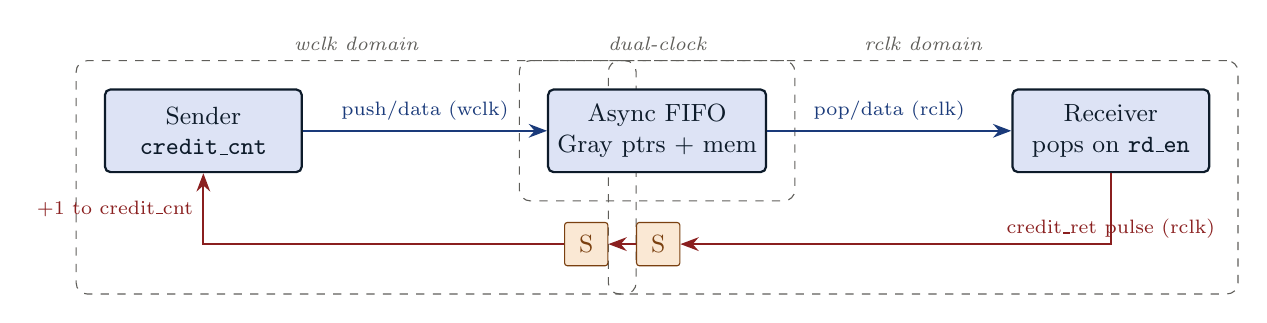
\begin{tikzpicture}[
  font=\small,
  blk/.style={draw=Navy, fill=BlueF, rounded corners=2pt, minimum height=1.05cm,
    minimum width=2.5cm, align=center, text=Navy, line width=0.8pt},
  reg/.style={draw=Amber, fill=AmberF, rounded corners=1pt, minimum height=0.55cm,
    minimum width=0.55cm, text=Amber},
  dom/.style={draw=MGray, dashed, rounded corners=4pt, inner sep=10pt},
  lbl/.style={font=\scriptsize\itshape, text=MGray},
  >=Stealth
]
  \node[blk] (sender) {Sender\\\texttt{credit\_cnt}};
  \node[blk, right=3.1cm of sender] (fifo) {Async FIFO\\Gray ptrs + mem};
  \node[blk, right=3.1cm of fifo] (receiver) {Receiver\\pops on \texttt{rd\_en}};

  \draw[->, Blue, thick] (sender.east) -- node[above,font=\scriptsize]{push/data (wclk)} (fifo.west);
  \draw[->, Blue, thick] (fifo.east) -- node[above,font=\scriptsize]{pop/data (rclk)} (receiver.west);

  \node[reg] (s1) at ($(fifo.south)+(-0.9,-0.9)$) {S};
  \node[reg, right=0.35cm of s1] (s2) {S};
  \draw[->, Red, thick] (receiver.south) |- node[pos=0.25,below,font=\scriptsize]
       {credit\_ret pulse (rclk)} (s2.east);
  \draw[->, Red, thick] (s2) -- (s1);
  \draw[->, Red, thick] (s1.west) -| node[pos=0.75,left,font=\scriptsize]
       {+1 to credit\_cnt} (sender.south);

  \begin{scope}[on background layer]
    \node[dom, fit=(sender)(s1), label={[lbl]above:wclk domain}] {};
    \node[dom, fit=(receiver)(s2), label={[lbl]above:rclk domain}] {};
    \node[dom, fit=(fifo), label={[lbl]above:dual-clock}] {};
  \end{scope}
\end{tikzpicture}
\end{center}
\begin{center}
\parbox{0.85\linewidth}{\footnotesize\color{MGray}
Forward path (push/data, pop/data) crosses through the FIFO memory itself,
gated by Gray-coded pointers (Section~\ref{sec:pointer}). The
\texttt{credit\_ret} pulse crosses back through its own 2-flop
synchronizer ("S"--"S" above) directly into the write domain's
\texttt{credit\_cnt} register — it does not go through the FIFO memory at
all, it is a side-band 1-bit signal.}
\end{center}

\subsection{Why a 1-bit pulse, and not the credit \emph{count} itself?}

An alternative design would have the receiver compute "credits currently
available" as a small bus (say, $\lceil\log_2 D\rceil$ bits) and send that
\emph{value} across to the sender, instead of a single accumulating pulse.
That alternative is strictly worse here, for reasons that follow directly
from Sections~\ref{sec:pointer} and \ref{sec:cdc}:

\begin{itemize}[leftmargin=1.4em]
  \item \textbf{A multi-bit value crossing domains has exactly the same
  torn-sample problem as the pointers do} (Section~\ref{sec:cdc}): if the
  available-credits bus changes by more than 1 bit between two samples,
  and the destination clock samples mid-transition, it can catch a
  combination of old and new bits that was never a value the counter
  actually held. Fixing that would mean Gray-coding the credit-count bus
  \emph{too} — solving a problem the pulse scheme never creates in the
  first place.
  \item \textbf{A pulse is inherently single-bit}, so the only CDC
  primitive it ever needs is the plain 2-flop synchronizer (plus the
  toggle/edge-detect wrapper for pulse-width safety, Section~\ref{sec:pulsesync}) — no
  Gray coding, no multi-bit comparison logic, nothing.
  \item \textbf{The arithmetic that matters (how many credits are left)
  stays entirely inside one clock domain} — the write domain's
  \texttt{credit\_cnt} register. The read domain never needs to know, or
  compute, "how many credits are available"; it only needs to notice,
  locally, "I just freed one slot," which is a fact it already has for
  free the instant it completes a pop. Moving a \emph{count} across
  domains would require the read side to maintain its own shadow copy of
  the write side's arithmetic, doubling the state that has to agree
  between domains for no benefit.
\end{itemize}

\begin{keybox}
General principle: whenever a quantity can be re-expressed as "count of
discrete, one-at-a-time events" instead of "a computed value," prefer
sending the \emph{events} (pulses) across a clock domain and doing the
arithmetic locally on one side. It collapses an $N$-bit CDC problem (which
needs Gray coding or an equivalent handshake) into an easier 1-bit CDC
problem (which only needs the standard synchronizer). This is precisely
the same trick, one level up, as Gray-coding the pointers themselves:
Section~\ref{sec:pointer}'s pointers are also "a count of discrete
push/pop events," just exposed as a running total rather than as
individual pulses -- and note they still need Gray coding for exactly the
reason a raw multi-bit credit count would.
\end{keybox}

% ============================================================
\section{Valid/Ready, recap}
% ============================================================

Standard synchronous handshake rules (matches AXI-style valid/ready):

\begin{enumerate}[leftmargin=1.4em]
  \item A transfer happens on any clock edge where \texttt{valid=1 AND
  ready=1} are sampled together.
  \item Once \texttt{valid} is asserted, the sender may \textbf{not}
  withdraw it (or change the data) until a transfer occurs.
  \item \texttt{ready} is allowed to be a combinational function of
  \texttt{valid} (receiver may say "I can take it, if you're offering") but
  \texttt{valid} must not combinationally depend on \texttt{ready} (no
  same-cycle "I'll only offer if you can take it" — that creates a
  combinational loop across the interface).
\end{enumerate}

This works perfectly when sender and receiver are point-to-point with
nothing but wires between them. The trouble starts the moment you insert
\textbf{registers} into either the forward (valid/data) path or the
backward (ready) path — which is exactly what happens whenever a pipeline
stage, a crossbar hop, or a pipelined memory sits in between. That is the
subject of the next section.

\subsection{Why can't \texttt{ready} just stay combinational everywhere?}

In principle nothing stops you wiring \texttt{ready} straight back
combinationally no matter how many stages sit in the forward path — Case~2
already showed a purely-forward-registered pipeline costs nothing, provided
the reverse path is still instantaneous. The reason real designs
\emph{can't} keep doing that indefinitely is physical, not logical:

\begin{itemize}[leftmargin=1.4em]
  \item \textbf{Timing closure.} A combinational \texttt{ready} that has to
  travel from the last stage of a deep pipeline all the way back to the
  first is one long combinational path, competing for the same clock
  period as every other path in the design. Once that path's delay
  approaches the clock period, the only fixes are slowing the clock down
  (usually unacceptable) or registering it (which is exactly what
  Sections~\ref{sec:cases} Cases 3--6 analyze).
  \item \textbf{Floorplan distance.} On real silicon the sender and
  receiver of a handshake are not colocated — a \texttt{ready} wire
  crossing a large block or a NoC hop has real wire delay, plus buffering
  insertion for signal integrity, both of which show up as pipeline
  \emph{stages} whether you asked for them or not.
  \item \textbf{Fan-out / fan-in.} A \texttt{ready} signal that has to be
  combinationally gated by many downstream consumers (e.g.\ an arbiter
  with several requestors) accumulates logic depth with every additional
  consumer, again eating into the same timing budget.
\end{itemize}

So registered handshake signals are not a design mistake to be avoided —
they are a structural consequence of building anything with real pipeline
depth or real floorplan distance. The question this document actually
answers is: \emph{given} that registers will end up in the round trip
somewhere, which handshake discipline degrades gracefully as they
accumulate, and which one requires a fresh, local, re-derived buffering
decision at every single stage. Section~\ref{sec:cases} works through both
side by side.

\clearpage
% ============================================================
\section{The 10 cases}
\label{sec:cases}
% ============================================================

Convention used in every waveform below: \texttt{clk} is a single shared
clock for all of Part~\ref{sec:cases} (we isolate the CDC problem to
Section~\ref{sec:cdc} — mixing both at once obscures which effect is
causing what). Each column is one clock cycle, numbered along the top.
Shaded cycles mark a \emph{lost} (stalled/bubbled) transfer opportunity.

% -------------------- CASE 1 --------------------
\begin{casebox}{Case 1 -- Valid/Ready, zero buffers (direct wire connect)}
Sender and receiver are directly wired: \texttt{valid} and \texttt{data} go
straight from sender output to receiver input, \texttt{ready} comes straight
back, both purely combinational (0 gate delay assumed for the diagram).

\begin{center}
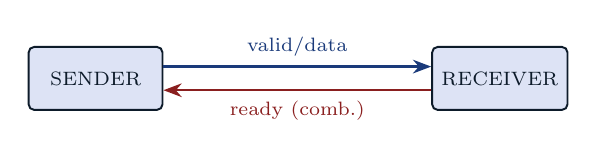
\begin{tikzpicture}[font=\scriptsize,
    blk/.style={draw=Navy,fill=BlueF,rounded corners=2pt,minimum height=0.8cm,
      minimum width=1.7cm,align=center,text=Navy,line width=0.7pt},
    >=Stealth]
  \node[blk] (S) {SENDER};
  \node[blk, right=3.4cm of S] (R) {RECEIVER};
  \draw[->,Blue,thick] ($(S.east)+(0,0.15)$) -- node[above]{valid/data}
       ($(R.west)+(0,0.15)$);
  \draw[->,Red,thick] ($(R.west)+(0,-0.15)$) -- node[below]{ready (comb.)}
       ($(S.east)+(0,-0.15)$);
\end{tikzpicture}
\end{center}

\begin{center}
\begin{tikztimingtable}[timing/rowdist=2.6ex, timing/wscale=0.85]
  clk    & 8{C} \\
  valid  & 6H L H \\
  ready  & 7H 1L \\
  data   & 3D{a} D{b} D{c} 2D{d} 1U \\
  xfer?  & 3D{Y} D{Y} D{Y} 2D{Y} 1D{-} \\
\end{tikztimingtable}
\end{center}

\textbf{Round trip: 0 cycles.} \texttt{ready} reflects the receiver's
\emph{true, current} state every cycle because there is no register between
"receiver decides" and "sender sees." Every cycle with \texttt{valid=1,
ready=1} transfers. No wasted cycles, no buffering needed. This is the
baseline everything else is measured against.
\end{casebox}

% -------------------- CASE 2 --------------------
\begin{casebox}{Case 2 -- Valid/Ready, 1 register in the forward (data/valid) path only}
A pipeline register is inserted \emph{after} the sender, before the
receiver, on \texttt{valid}/\texttt{data} only. \texttt{ready} still runs
straight back from receiver to that register's enable (no register on the
reverse path).

\begin{center}
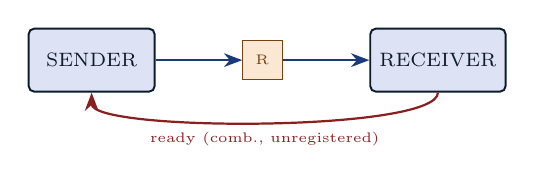
\begin{tikzpicture}[font=\scriptsize,
    blk/.style={draw=Navy,fill=BlueF,rounded corners=2pt,minimum height=0.8cm,
      minimum width=1.6cm,align=center,text=Navy,line width=0.7pt},
    reg/.style={draw=Amber,fill=AmberF,minimum height=0.5cm,minimum width=0.5cm,
      text=Amber,font=\tiny},
    >=Stealth]
  \node[blk] (S) {SENDER};
  \node[reg, right=1.1cm of S] (Ff) {R};
  \node[blk, right=1.1cm of Ff] (R) {RECEIVER};
  \draw[->,Blue,thick] (S) -- (Ff);
  \draw[->,Blue,thick] (Ff) -- (R);
  \draw[->,Red,thick] (R.south) .. controls +(0,-0.5) and +(0,-0.5) .. (S.south)
    node[midway,below,font=\tiny]{ready (comb., unregistered)};
\end{tikzpicture}
\end{center}

\begin{center}
\begin{tikztimingtable}[timing/rowdist=2.6ex, timing/wscale=0.85]
  clk         & 8{C} \\
  valid$_{in}$& 6H L H \\
  ready$_{rx}$& 8H \\
  valid$_{reg}$ (+1cyc) & L 6H L \\
  data$_{reg}$          & 1U 3D{a} D{b} D{c} 2D{d} \\
\end{tikztimingtable}
\end{center}

Because \texttt{ready} is still combinational from the true receiver state,
and the register has an enable tied to that same \texttt{ready} (it holds
its value if the receiver isn't ready, i.e.\ it is really a 1-deep skid
register, not a blind pipeline flop), \textbf{no throughput is lost} — this
case just adds 1 cycle of pure latency, not a round trip. This is the
"safe" direction to add a register: forward-path registers only ever cost
latency, never bandwidth, \emph{provided} the register has a proper stall/
hold-if-not-ready enable.
\end{casebox}

% -------------------- CASE 3 --------------------
\begin{casebox}{Case 3 -- Valid/Ready, 1 register in the backward (ready) path only}
Now flip it: \texttt{valid}/\texttt{data} run straight through combinationally,
but the receiver's \texttt{ready} is registered before it reaches the sender.
This is the dangerous direction.

\begin{center}
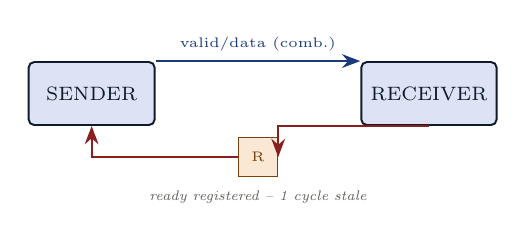
\begin{tikzpicture}[font=\scriptsize,
    blk/.style={draw=Navy,fill=BlueF,rounded corners=2pt,minimum height=0.8cm,
      minimum width=1.6cm,align=center,text=Navy,line width=0.7pt},
    reg/.style={draw=Amber,fill=AmberF,minimum height=0.5cm,minimum width=0.5cm,
      text=Amber,font=\tiny},
    >=Stealth]
  \node[blk] (S) {SENDER};
  \node[blk, right=2.6cm of S] (R) {RECEIVER};
  \path (S) -- (R) coordinate[midway] (mid);
  \node[reg, below=0.55cm of mid] (Fb) {R};
  \draw[->,Blue,thick] (S.north east) -- node[above,font=\tiny]{valid/data (comb.)} (R.north west);
  \draw[->,Red,thick] (R.south) -| (Fb.east);
  \draw[->,Red,thick] (Fb.west) -| (S.south);
  \node[below=0.05cm of Fb, font=\tiny\itshape, text=MGray]{ready registered -- 1 cycle stale};
\end{tikzpicture}
\end{center}

\begin{center}
\begin{tikztimingtable}[timing/rowdist=2.6ex, timing/wscale=0.85]
  clk              & 8{C} \\
  ready$_{true}$   & 3H L 4H \\
  ready$_{sender}$ (+1cyc, stale) & L 3H L 4H \\
  valid            & 2H L 5H \\
  \# xfer claimed  & 1D{-} D{Y} D{Y} D{-} 4D{Y} \\
\end{tikztimingtable}
\end{center}

\begin{warnbox}
At cycle~4 the sender is looking at \texttt{ready\_sender}, which is
\emph{last cycle's} answer (still high), and sends. But the receiver's
\emph{true} state at cycle~4 has already dropped to not-ready. The sender's
data is accepted into a receiver that has no room — data corruption/overrun,
unless the receiver over-provisions a landing buffer (a skid register) to
catch that one "in-flight" beat. \textbf{A registered ready signal is only
safe if the receiver keeps at least 1 extra slot of storage to absorb
whatever was already committed to fly before the stale ready was seen.}
This is the first hint that pure valid/ready starts needing extra buffering
the moment either direction is registered.
\end{warnbox}
\end{casebox}

% -------------------- CASE 4 --------------------
\begin{casebox}{Case 4 -- Valid/Ready, 1 register in \emph{both} directions (round trip = 2)}
Now both paths are registered: \texttt{valid/data} take 1 cycle to arrive,
\texttt{ready} takes 1 cycle to return. A change in receiver state takes
\textbf{2 cycles} (1 out, 1 back) to be reflected in what the sender sees.

\begin{center}
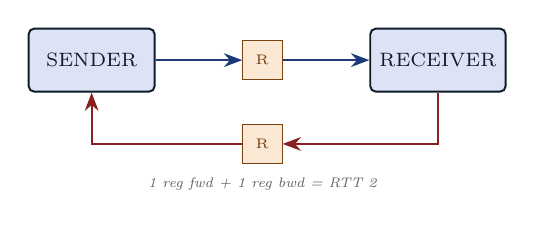
\begin{tikzpicture}[font=\scriptsize,
    blk/.style={draw=Navy,fill=BlueF,rounded corners=2pt,minimum height=0.8cm,
      minimum width=1.6cm,align=center,text=Navy,line width=0.7pt},
    reg/.style={draw=Amber,fill=AmberF,minimum height=0.5cm,minimum width=0.5cm,
      text=Amber,font=\tiny},
    >=Stealth]
  \node[blk] (S) {SENDER};
  \node[reg, right=1.1cm of S] (Ff) {R};
  \node[blk, right=1.1cm of Ff] (R) {RECEIVER};
  \node[reg, below=0.55cm of Ff] (Fb) {R};
  \draw[->,Blue,thick] (S) -- (Ff);
  \draw[->,Blue,thick] (Ff) -- (R);
  \draw[->,Red,thick] (R.south) |- (Fb.east);
  \draw[->,Red,thick] (Fb.west) -| (S.south);
  \node[below=0.05cm of Fb, font=\tiny\itshape, text=MGray]{1 reg fwd + 1 reg bwd = RTT 2};
\end{tikzpicture}
\end{center}

\begin{center}
\begin{tikztimingtable}[timing/rowdist=2.6ex, timing/wscale=0.85]
  clk                 & 10{C} \\
  valid$_{sent}$      & 4H 2L 4H \\
  ready$_{seen}$(t-2) & 2H 2L 2H 2L 2H \\
  \# actually accepted& 2D{Y}2D{-}2D{Y}2D{-}2D{Y} \\
\end{tikztimingtable}
\end{center}

Without any local buffering, every time the receiver's true state flips,
the sender is working off information that is 2 cycles stale, so it must
either (a) conservatively stop sending the instant it \emph{might} be wrong
— losing throughput it didn't need to lose — or (b) risk overrunning like
Case~3, now for up to 2 beats in flight instead of 1.

\begin{formulabox}
To sustain full 1-transfer/cycle throughput safely with a 2-cycle round
trip, the receiver-side landing buffer must hold \textbf{at least 2}
in-flight beats (skid depth = round trip in cycles). This is exactly why
registered-ready designs pair every extra pipeline stage with extra skid
storage.
\end{formulabox}
\end{casebox}

% -------------------- CASE 5 --------------------
\begin{casebox}{Case 5 -- Valid/Ready, 2 registers each direction (round trip = 4)}
Same structure, doubled: 2 forward registers, 2 backward registers. Round
trip is now $2+2=4$ cycles.

\begin{center}
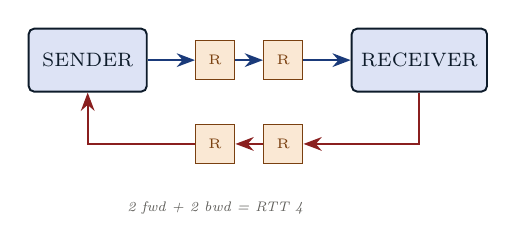
\begin{tikzpicture}[font=\scriptsize,
    blk/.style={draw=Navy,fill=BlueF,rounded corners=2pt,minimum height=0.8cm,
      minimum width=1.5cm,align=center,text=Navy,line width=0.7pt},
    reg/.style={draw=Amber,fill=AmberF,minimum height=0.5cm,minimum width=0.5cm,
      text=Amber,font=\tiny},
    >=Stealth]
  \node[blk] (S) {SENDER};
  \node[reg, right=0.6cm of S] (F1) {R};
  \node[reg, right=0.35cm of F1] (F2) {R};
  \node[blk, right=0.6cm of F2] (R) {RECEIVER};
  \node[reg, below=0.55cm of F2] (B2) {R};
  \node[reg, left=0.35cm of B2] (B1) {R};
  \draw[->,Blue,thick] (S) -- (F1);
  \draw[->,Blue,thick] (F1) -- (F2);
  \draw[->,Blue,thick] (F2) -- (R);
  \draw[->,Red,thick] (R.south) |- (B2.east);
  \draw[->,Red,thick] (B2) -- (B1);
  \draw[->,Red,thick] (B1.west) -| (S.south);
  \node[below=0.35cm of B1, font=\tiny\itshape, text=MGray]{2 fwd + 2 bwd = RTT 4};
\end{tikzpicture}
\end{center}

\begin{center}
\begin{tikztimingtable}[timing/rowdist=2.6ex, timing/wscale=0.85]
  clk                 & 12{C} \\
  valid$_{sent}$      & 6H 4L 2H \\
  ready$_{seen}$(t-4) & 4H 4L 4H \\
\end{tikztimingtable}
\end{center}

Skid depth required to not lose throughput: \textbf{4}. Notice the pattern:
\emph{every} register you add anywhere in either direction directly adds to
required buffering elsewhere, linearly, forever. There is no amount of
"just add one more pipeline stage for timing closure" that comes for free
under valid/ready once you care about sustained throughput.
\end{casebox}

% -------------------- CASE 6 --------------------
\begin{casebox}{Case 6 -- Valid/Ready, generalized to N registers each direction}
\begin{center}
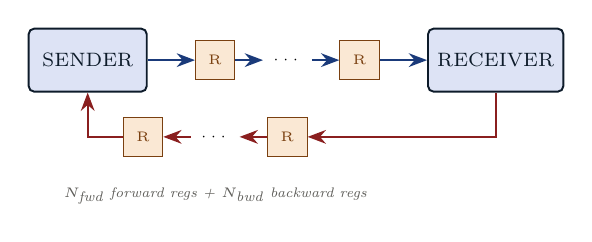
\begin{tikzpicture}[font=\scriptsize,
    blk/.style={draw=Navy,fill=BlueF,rounded corners=2pt,minimum height=0.8cm,
      minimum width=1.5cm,align=center,text=Navy,line width=0.7pt},
    reg/.style={draw=Amber,fill=AmberF,minimum height=0.5cm,minimum width=0.5cm,
      text=Amber,font=\tiny},
    >=Stealth]
  \node[blk] (S) {SENDER};
  \node[reg, right=0.6cm of S] (F1) {R};
  \node[right=0.35cm of F1, font=\tiny] (dots1) {$\cdots$};
  \node[reg, right=0.35cm of dots1] (Fn) {R};
  \node[blk, right=0.6cm of Fn] (R) {RECEIVER};
  \node[reg, below=0.55cm of dots1] (B1) {R};
  \node[left=0.35cm of B1, font=\tiny] (dots2) {$\cdots$};
  \node[reg, left=0.35cm of dots2] (Bn) {R};
  \draw[->,Blue,thick] (S) -- (F1);
  \draw[->,Blue,thick] (F1) -- (dots1);
  \draw[->,Blue,thick] (dots1) -- (Fn);
  \draw[->,Blue,thick] (Fn) -- (R);
  \draw[->,Red,thick] (R.south) |- (B1.east);
  \draw[->,Red,thick] (B1) -- (dots2);
  \draw[->,Red,thick] (dots2) -- (Bn);
  \draw[->,Red,thick] (Bn.west) -| (S.south);
  \node[below=0.35cm of dots2, font=\tiny\itshape, text=MGray]
    {$N_{\text{fwd}}$ forward regs + $N_{\text{bwd}}$ backward regs};
\end{tikzpicture}
\end{center}
\[
  \text{RTT}_{\text{cycles}} = N_{\text{fwd}} + N_{\text{bwd}}
  \qquad
  \text{skid depth to sustain full throughput} \;\geq\; \text{RTT}_{\text{cycles}}
\]
This is the structural reason valid/ready is disfavored once a datapath has
real pipeline depth in it: \textbf{every} stage added for timing closure
(placement, routing, clock period) must be matched \emph{locally, at that
exact stage} by enough skid storage to cover the round trip back to
whoever is asserting \texttt{valid}. That storage decision is smeared across
every stage of the design, has to be re-derived every time the pipeline is
re-pipelined, and each skid buffer duplicates state (valid/data storage)
that a single, centrally-sized FIFO could have held once. This is the
"why not preferred" answer.
\end{casebox}

\clearpage
Now the credit-based equivalents of the same topologies.

% -------------------- CASE 7 --------------------
\begin{casebox}{Case 7 -- Valid/Credit, zero buffers (baseline, matches Case 1)}
\texttt{credit\_cnt} initialized to FIFO depth $D$ at reset. Sender pushes
whenever \texttt{credit\_cnt}$>0$; receiver pulses \texttt{credit\_ret} every
cycle it pops.

\begin{center}
\begin{tikztimingtable}[timing/rowdist=2.6ex, timing/wscale=0.85]
  clk          & 6{C} \\
  push         & 6H \\
  pop          & 6H \\
  credit\_ret  & 6H \\
  credit\_cnt  & D{D}D{D}D{D}D{D}D{D}D{D} \\
\end{tikztimingtable}
\end{center}

With zero physical latency, push and credit-return are same-cycle events —
counter never actually moves, it's degenerate, and behaves identically to
Case~1. This just establishes the counter's steady state.
\end{casebox}

% -------------------- CASE 8 --------------------
\begin{casebox}{Case 8 -- Valid/Credit, registers in both directions (round trip = 2, matches Case 4's topology)}
Same physical pipeline as Case~4 — 1 register each direction — but now the
backward signal is a \emph{credit pulse}, not a live "state" signal, and the
sender is driven by its own counter, not by a stale copy of receiver state.

\begin{center}
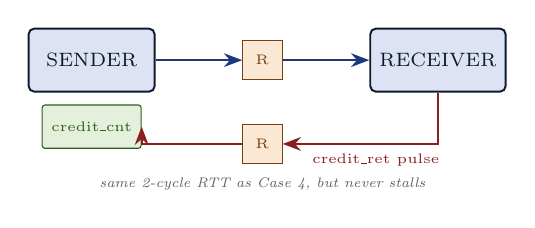
\begin{tikzpicture}[font=\scriptsize,
    blk/.style={draw=Navy,fill=BlueF,rounded corners=2pt,minimum height=0.8cm,
      minimum width=1.6cm,align=center,text=Navy,line width=0.7pt},
    cnt/.style={draw=Green,fill=GreenF,rounded corners=1pt,minimum height=0.55cm,
      minimum width=1.2cm,text=Green,font=\tiny},
    reg/.style={draw=Amber,fill=AmberF,minimum height=0.5cm,minimum width=0.5cm,
      text=Amber,font=\tiny},
    >=Stealth]
  \node[blk] (S) {SENDER};
  \node[cnt, below=0.15cm of S] (C) {credit\_cnt};
  \node[reg, right=1.1cm of S] (Ff) {R};
  \node[blk, right=1.1cm of Ff] (R) {RECEIVER};
  \node[reg, below=0.55cm of Ff] (Fb) {R};
  \draw[->,Blue,thick] (S) -- (Ff);
  \draw[->,Blue,thick] (Ff) -- (R);
  \draw[->,Red,thick] (R.south) |- node[pos=0.7,below,font=\tiny]{credit\_ret pulse}(Fb.east);
  \draw[->,Red,thick] (Fb.west) -| (C.east);
  \node[below=0.05cm of Fb, font=\tiny\itshape, text=MGray]{same 2-cycle RTT as Case 4, but never stalls};
\end{tikzpicture}
\end{center}

\begin{center}
\begin{tikztimingtable}[timing/rowdist=2.6ex, timing/wscale=0.85]
  clk           & 10{C} \\
  push          & 10H \\
  credit\_cnt   & D{4}D{3}D{2}D{1}D{0}D{1}D{0}D{1}D{0}D{1} \\
  credit\_ret(+2cyc) & 2L H L H L H L H L H \\
\end{tikztimingtable}
\end{center}

Sender \textbf{never stalls} as long as $D \geq$ RTT: it keeps pushing every
cycle (draining the pre-loaded counter), and by the time the counter would
hit 0 for good, credit pulses from 2 cycles ago are already flowing back to
replenish it at the same steady-state rate. \textbf{The round trip latency
is still physically there} (2 cycles, unchanged) — it just never shows up
as a stall, because it was pre-paid for by the initial credit balance
(= the FIFO depth) instead of being discovered live.
\end{casebox}

% -------------------- CASE 9 --------------------
\begin{casebox}{Case 9 -- Valid/Credit, generalized to N registers each direction}
\begin{formulabox}
\[
  D_{\min} \;\geq\; \text{RTT}_{\text{cycles}} \times \text{(max sustained push rate, in pushes/cycle)}
\]
For a 1-push-per-cycle producer, $D_{\min} \geq \text{RTT}_{\text{cycles}}$
exactly (Section~\ref{sec:sizing} adds a +1 guard entry and CDC terms on
top of this). \textbf{Depth absorbs latency; latency never has to be
discovered live.} This is why credit interfaces scale to arbitrarily deep
pipelines without touching per-stage logic — every extra register anywhere
in the round trip just raises one number (required depth) at the one place
that already owns storage (the FIFO), instead of demanding a new skid
buffer at every stage.
\end{formulabox}
\end{casebox}

% -------------------- CASE 10 --------------------
\begin{casebox}{Case 10 -- Valid/Credit, \emph{under-sized} depth ($D < $ RTT)}
Take Case~8's exact 2-cycle-RTT pipeline, but set $D=1$ instead of $D\geq 2$.

\begin{center}
\begin{tikztimingtable}[timing/rowdist=2.6ex, timing/wscale=0.85]
  clk           & 8{C} \\
  push          & 8H \\
  credit\_cnt   & D{1}D{0}D{X}D{X}D{X}D{X}D{X}D{X} \\
  credit\_ret(+2cyc) & 2L H L H L H L H \\
\end{tikztimingtable}
\end{center}

\begin{warnbox}
At cycle~2, \texttt{credit\_cnt} is already 0, but \texttt{push} is still
asserted (nothing told the sender to stop — that \emph{is} the point of a
credit scheme, it doesn't ask, it counts). If the counter is allowed to go
negative / wrap (marked \texttt{X} above), the sender believes it has
credit it doesn't, and the physical FIFO — which really is full — gets
written anyway: the write pointer catches and passes the read pointer,
\textbf{silently overwriting an entry the reader has not consumed yet}.
This is the credit-interface equivalent of Case~3's overrun, and it is
strictly a \emph{sizing} bug, not a protocol bug: the fix is always
$D \geq \text{RTT}$, never "add more handshake logic."
\end{warnbox}

\textbf{The opposite mistake — over-sizing} ($D \gg$ RTT) costs silicon
area (deeper memory, wider pointers) but, unlike valid/ready's registered
case, \textbf{costs zero bandwidth}: the counter just idles higher on
average. Contrast this directly with Case~6: in valid/ready, insufficient
skid buffering directly steals throughput every cycle it's short; in
valid/credit, insufficient depth corrupts data (a much worse, and much more
detectable-in-verification, failure) while correct-or-generous depth always
gives full throughput. \textbf{There is no "wasted bandwidth from
oversizing" in a credit scheme} — that penalty is unique to under-buffered
valid/ready pipelines, which is precisely why "how much skid do I need"
questions disappear once you centralize storage sizing into one FIFO depth
number.
\end{casebox}

\clearpage
% ============================================================
\section{Depth sizing formulas}
\label{sec:sizing}
% ============================================================

\subsection{Same-clock round trip (Section~\ref{sec:cases} recap)}
\[
D_{\min} = \big\lceil \text{RTT}_{\text{cycles}} \big\rceil + 1
\]
The $+1$ is a guard entry: it covers the boundary case where the last
credit-consuming push and the first credit-return pulse land on adjacent
cycles with no double-counting margin, and is cheap insurance relative to
re-deriving exact fencepost arithmetic per design.

\subsection{Cross-clock round trip (the real async-FIFO case)}
\label{sec:sizing-cdc}

Now the credit pulse must itself cross a clock domain (read domain, where
it's generated, back into write domain, where the counter lives), through a
standard 2-flop synchronizer (justified in Section~\ref{sec:cdc}). Break
the round trip into its physical pieces, each measured \emph{in write-clock
cycles} since that's the domain the counter lives in and the domain that
must not overflow:

\begin{center}
\begin{tabular}{@{}p{5.6cm}p{9.6cm}@{}}
\toprule
\textbf{Segment} & \textbf{Latency (write-clock cycles)} \\
\midrule
Write $\to$ read domain crossing of the data/valid path (if the write
pointer or data itself must be observed in read domain before a pop can
happen) & $2 \times T_{rclk}/T_{wclk}$ (2-flop sync, converted) \\
Any pipeline registers purely inside the read domain before the pop
completes & $N_{read\_pipe} \times T_{rclk}/T_{wclk}$ \\
Read $\to$ write domain crossing of the credit-return pulse (2-flop sync,
this time the destination clock \emph{is} \texttt{wclk} so no conversion
needed) & $2$ \\
Any pipeline registers purely inside the write domain after credit is
received & $N_{write\_pipe}$ \\
\bottomrule
\end{tabular}
\end{center}

\begin{formulabox}
\[
D_{\min} \;\geq\; \left\lceil 2\cdot\frac{T_{rclk}}{T_{wclk}} + N_{read\_pipe}\cdot\frac{T_{rclk}}{T_{wclk}}
\;+\; 2 \;+\; N_{write\_pipe} \right\rceil \;+\; 1
\]
all evaluated in write-clock cycle units, because the write side is the one
whose overflow you must prevent and whose counter is ticking at
$T_{wclk}$.
\end{formulabox}

\subsubsection{Worked example -- write faster than read (\texttt{wclk}=200\,MHz, \texttt{rclk}=100\,MHz)}
$T_{rclk}/T_{wclk} = 2$. Assume no extra pipe stages either side
($N_{read\_pipe}=N_{write\_pipe}=0$):
\[
D_{\min} \geq \lceil 2\cdot2 + 0 + 2 + 0\rceil + 1 = 6+1 = 7 \;\Rightarrow\; \text{round up to } D=8.
\]
\textbf{Intuition:} every single read-domain cycle, up to 2 write-domain
cycles' worth of pushes can occur (write is 2$\times$ faster), so any
latency measured in read cycles must be inflated by that ratio before it's
counted against the write-side counter. This is \emph{why write-faster-
than-read is the sizing-sensitive direction}: the producer can burn through
credit much faster than the consumer's acknowledgements can be generated
and relayed back, so the buffer has to be deep enough to cover that whole
window at the fast rate.

\subsubsection{Worked example -- read faster than write (\texttt{wclk}=100\,MHz, \texttt{rclk}=200\,MHz)}
$T_{rclk}/T_{wclk} = 0.5$:
\[
D_{\min} \geq \lceil 2\cdot0.5 + 0 + 2 + 0\rceil + 1 = 3+1 = 4.
\]
\textbf{Intuition:} the read domain issues its credit-return pulse (and, if
applicable, observes the write pointer) at a rate faster than the producer
can consume credit, so the synchronizer latency — while still physically
2--3 read-domain cycles — represents \emph{less} write-domain-cycle
"damage window." \textbf{You still need the 2-flop synchronizer either
way} (metastability doesn't care about clock ratio), but the depth penalty
from that latency shrinks because the write side, which is the slower
producer, simply can't burn through many credits before the faster domain
catches up. \textbf{Do not skip sizing analysis just because read is
faster} — always compute $D_{\min}$ from the formula; it's smaller here,
not absent.

\subsubsection{Sizing sweep across clock ratios}

Same formula ($N_{read\_pipe}=N_{write\_pipe}=0$), swept across common
ratios, to show the trend rather than just two endpoints:

\begin{center}
\renewcommand{\arraystretch}{1.2}
\begin{tabular}{ccccc}
\toprule
\texttt{wclk} & \texttt{rclk} & $T_{rclk}/T_{wclk}$ & raw $D_{\min}$ (pre-round) & final $D_{\min}$ \\
\midrule
400\,MHz & 100\,MHz & 4.0 & $2(4)+2+1=11$ & 12 (round to pow2: 16) \\
266\,MHz & 100\,MHz & 2.66 & $2(2.66)+2+1=8.3$ & 9 (pow2: 16) \\
200\,MHz & 100\,MHz & 2.0 & $2(2)+2+1=7$ & 7 (pow2: 8) \\
100\,MHz & 100\,MHz & 1.0 & $2(1)+2+1=5$ & 5 (pow2: 8) \\
100\,MHz & 200\,MHz & 0.5 & $2(0.5)+2+1=4$ & 4 (pow2: 4) \\
100\,MHz & 400\,MHz & 0.25 & $2(0.25)+2+1=3.5$ & 4 (pow2: 4) \\
\bottomrule
\end{tabular}
\end{center}

Notice $D_{\min}$ \textbf{never drops below $\sim$3--4} even in the most
read-favorable ratio shown — that floor is the synchronizer latency itself
(the "$2+2$" fixed cost in the formula, from the two independent 2-flop
crossings in each direction), which is a fixed number of cycles regardless
of clock ratio. Only the write-faster-than-read term
($2 \cdot T_{rclk}/T_{wclk}$) actually grows with ratio, which is why that
direction dominates the sizing decision once the ratio departs from~1.

\begin{keybox}
Rule of thumb: \textbf{write-faster-than-read} is the sizing-critical
direction (deep buffer, size for it explicitly); \textbf{read-faster-than-
write} is comparatively forgiving (shallow minimum), but the synchronizer
latency itself, and therefore \emph{some} nonzero minimum depth, is never
optional in either direction.
\end{keybox}

\subsection{Cycle-by-cycle trace: correct depth vs.\ under-sized depth}
\label{sec:trace}

Take the 200/100\,MHz worked example: fixed round-trip latency
$\text{RTT}=6$ write-clock cycles between a push and its matching
\texttt{credit\_ret} arriving back (this folds together the read-domain
sync, the read-domain pipe, and the write-domain sync from
Section~\ref{sec:sizing-cdc}). Sender pushes every cycle whenever
\texttt{credit\_cnt}$>0$. All values below are in write-clock cycles.

\subsubsection{Correctly sized, $D=8 \geq \text{RTT}=6$}

\begin{center}\small
\renewcommand{\arraystretch}{1.05}
\begin{tabular}{cccccl}
\toprule
cyc & push? & wptr (dec) & credit\_ret? & rptr (dec, $=$wptr$-$RTT) & credit\_cnt \\
\midrule
0  & Y & 1  & -- & 0 & 7 \\
1  & Y & 2  & -- & 0 & 6 \\
2  & Y & 3  & -- & 0 & 5 \\
3  & Y & 4  & -- & 0 & 4 \\
4  & Y & 5  & -- & 0 & 3 \\
5  & Y & 6  & -- & 0 & 2 \\
6  & Y & 7  & Y (from cyc 0) & 1 & 2 \\
7  & Y & 8  & Y (from cyc 1) & 2 & 2 \\
8  & Y & 9  & Y (from cyc 2) & 3 & 2 \\
9  & Y & 10 & Y (from cyc 3) & 4 & 2 \\
10 & Y & 11 & Y (from cyc 4) & 5 & 2 \\
\bottomrule
\end{tabular}
\end{center}

After the initial 6-cycle fill (unavoidable — those credits are what the
depth exists to pre-pay for), \texttt{credit\_cnt} settles at a steady-state
floor of $D-\text{RTT}=8-6=2$ and \textbf{never reaches 0}: push continues
every single cycle, forever, at full 1/cycle throughput. This is the
"correctly sized" outcome — the floor value (2, here) is your actual margin
above the minimum; it is what the "+1 guard / round to next power of 2"
step in the formula bought you.

\subsubsection{Under-sized, correctly gated, $D=1 < \text{RTT}=6$}

\begin{center}\small
\renewcommand{\arraystretch}{1.05}
\begin{tabular}{cccccl}
\toprule
cyc & push? & wptr (dec) & credit\_ret? & credit\_cnt & note \\
\midrule
0 & Y & 1 & -- & 0 & only credit spent immediately \\
1 & \cellcolor{RedF}N & 1 & -- & 0 & \cellcolor{RedF}stalled -- no credit \\
2 & \cellcolor{RedF}N & 1 & -- & 0 & \cellcolor{RedF}stalled \\
3 & \cellcolor{RedF}N & 1 & -- & 0 & \cellcolor{RedF}stalled \\
4 & \cellcolor{RedF}N & 1 & -- & 0 & \cellcolor{RedF}stalled \\
5 & \cellcolor{RedF}N & 1 & -- & 0 & \cellcolor{RedF}stalled \\
6 & Y & 2 & Y (from cyc 0) & 0 & credit arrives, spent same cycle \\
7--11 & N & 2 & -- & 0 & stalled again, 5 more cycles \\
12 & Y & 3 & Y (from cyc 6) & 0 & pattern repeats, period 6 \\
\bottomrule
\end{tabular}
\end{center}

\textbf{No data corruption} — \texttt{push\_gnt} correctly stays low
whenever \texttt{credit\_cnt}$=0$ — but throughput has collapsed to
\textbf{1 push every 6 cycles (1/6 utilization)}. This is the concrete
version of the "over-skid/under-depth wastes bandwidth" statement from
Case~10: a \emph{correctly gated} but under-sized credit interface fails
safe, at the cost of most of its bandwidth, in direct proportion to how far
short of RTT the depth falls.

\subsubsection{Under-sized, \emph{incorrectly} gated (the bug), $D=1$}

Now suppose \texttt{credit\_cnt} is unsigned and the gating check was
written wrong (e.g.\ checked \texttt{push\_req} only, or the counter is
allowed to wrap instead of floor at 0) — a real bug class, not a
hypothetical:

\begin{center}\small
\renewcommand{\arraystretch}{1.05}
\begin{tabular}{ccccl}
\toprule
cyc & push? & wptr (dec) & phys.\ addr ($=$wptr mod $D{=}1$) & note \\
\midrule
0 & Y & 1 & 0 & data A written to the only slot \\
1 & Y & 2 & \cellcolor{RedF}0 & \cellcolor{RedF}data B overwrites A -- reader hasn't even been signaled (credit\_ret for cyc 0 doesn't land until cyc 6) \\
2 & Y & 3 & \cellcolor{RedF}0 & data C overwrites B, same story \\
\bottomrule
\end{tabular}
\end{center}

\begin{warnbox}
With physical depth 1 and a 6-cycle round trip, the \emph{very next} push
after the first one already lands on the same physical address before the
first entry has any chance of being popped — corruption isn't a rare
corner case here, it's the \emph{first} additional push. This is why
Section~\ref{sec:sizing}'s formula is a hard floor, not a suggestion: an
incorrectly-gated under-sized design doesn't degrade gracefully at all, it
corrupts data on the second beat.
\end{warnbox}

\clearpage
% ============================================================
\section{Pointer width: why \texttt{[N:0]}, not \texttt{[N-1:0]}}
\label{sec:pointer}
% ============================================================

For a FIFO of depth $2^{N}$ entries, indexing the memory only needs $N$
bits (\texttt{[N-1:0]}) — that addresses all $2^N$ locations. But the
read/write \emph{pointers} used for full/empty detection are kept
\textbf{one bit wider}, \texttt{[N:0]}, on purpose.

\begin{warnbox}
\textbf{Why \texttt{[N-1:0]} alone is ambiguous.} With only $N$ bits, the
write pointer wraps from $2^N-1$ back to $0$ exactly where it started.
After a full lap, \texttt{wptr == rptr} again — but that's \emph{also}
exactly the condition for "FIFO is empty" (no pushes have happened yet). An
$N$-bit-only pointer scheme cannot distinguish "completely full" from
"completely empty" — both present as \texttt{wptr == rptr}.
\end{warnbox}

\textbf{The fix:} widen both pointers to $N{+}1$ bits. The extra MSB acts
as a \textbf{wrap/lap counter} — it toggles every time the pointer wraps
around the physical memory. The bottom $N$ bits still address the memory
normally; the extra bit is only ever compared, never used to index.

\[
\text{empty} \;=\; (\text{wptr}_{\text{sync}} \;=\; \text{rptr})
\qquad
\text{full} \;=\; \big(\text{wptr}[N] \neq \text{rptr}_{\text{sync}}[N]\big)
\;\wedge\;
\big(\text{wptr}[N-1:0] = \text{rptr}_{\text{sync}}[N-1:0]\big)
\]

Reading this: \emph{same} bottom bits with the \emph{same} MSB means the
read pointer has caught all the way up to the write pointer on the
\emph{same lap} — empty. \emph{Same} bottom bits with a \emph{different}
MSB means the write pointer has lapped the read pointer exactly once and
is now bumping into it from behind — full. That single extra bit is the
entire mechanism that disambiguates the two, and it's why every real async
FIFO design (including the reference article this note builds on) always
carries pointers one bit wider than the address it decodes.

% ============================================================
\clearpage
\section{Clock domain crossing and metastability}
\label{sec:cdc}
% ============================================================

\subsection{Why crossing domains is dangerous at all}

A flip-flop needs its data input to be stable for a \textbf{setup time}
before, and a \textbf{hold time} after, the active clock edge. A signal
generated in a foreign, asynchronous clock domain has \emph{no}
relationship to the sampling clock's edges — sooner or later, purely by
chance, it will switch \emph{during} that setup/hold window.

When that happens, the flip-flop's internal storage node doesn't cleanly
resolve to a valid 0 or 1 in time. It sits balanced near the switching
threshold — physically, the two cross-coupled inverters that form the
latch are both trying to reinforce a voltage that's ambiguous to both of
them. This is \textbf{metastability}: an analog voltage sitting near
$V_{dd}/2$, not a "wrong digital value," an \emph{undefined} one, that only
resolves (settles fully high or fully low) after some — not fixed! —
amount of additional time.

\begin{center}
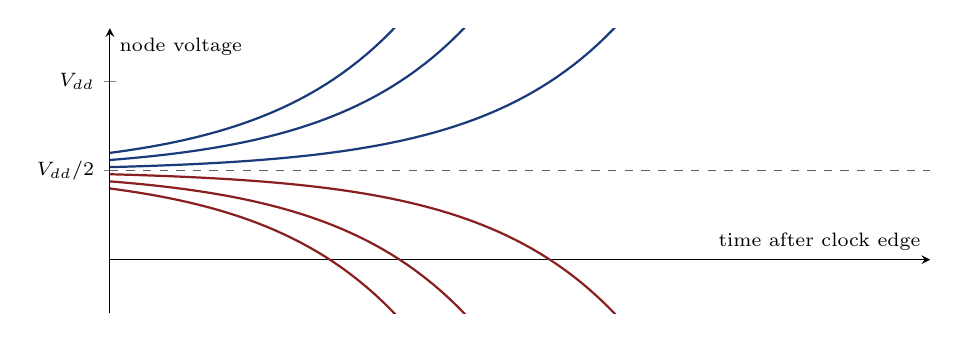
\begin{tikzpicture}[scale=1.0]
  \begin{axis}[
      width=12cm, height=5.2cm,
      xlabel={time after clock edge}, ylabel={node voltage},
      ymin=-0.3, ymax=1.3, xmin=0, xmax=6,
      axis lines=middle, ytick={0,0.5,1}, yticklabels={$0$,$V_{dd}/2$,$V_{dd}$},
      xtick=\empty, ylabel style={font=\scriptsize}, xlabel style={font=\scriptsize},
      tick label style={font=\scriptsize}, clip mode=individual,
      restrict y to domain=-0.35:1.35,
    ]
    % bundle of trajectories that "fan out" from near the threshold --
    % the classic metastability "bow-tie" picture: many trials, all
    % starting near 0.5, diverge exponentially to 0 or 1 depending on
    % which side of an infinitesimally unstable balance point they began.
    % restrict y to domain clips each trajectory once it saturates near
    % the rail, instead of letting the raw exponential blow up the bbox.
    \addplot[Blue, thick, domain=0:6, samples=100, unbounded coords=jump] {0.5 + 0.02*exp(x)};
    \addplot[Blue, thick, domain=0:6, samples=100, unbounded coords=jump] {0.5 + 0.06*exp(x)};
    \addplot[Blue, thick, domain=0:6, samples=100, unbounded coords=jump] {0.5 + 0.1*exp(x)};
    \addplot[Red,  thick, domain=0:6, samples=100, unbounded coords=jump] {0.5 - 0.02*exp(x)};
    \addplot[Red,  thick, domain=0:6, samples=100, unbounded coords=jump] {0.5 - 0.06*exp(x)};
    \addplot[Red,  thick, domain=0:6, samples=100, unbounded coords=jump] {0.5 - 0.1*exp(x)};
    \addplot[MGray, dashed] coordinates {(0,0.5) (6,0.5)};
  \end{axis}
\end{tikzpicture}
\captionof{figure}{The metastability "bow-tie": trajectories that begin
  infinitesimally above or below the exact balance threshold diverge
  \emph{exponentially} in time toward a valid \texttt{1} (blue) or
  \texttt{0} (red). Trajectories starting closer to the threshold take
  longer to resolve; there is no fixed worst-case bound, only a
  probability that shrinks the longer you wait.}
\end{center}

This exponential divergence is exactly why synchronizer design is
probabilistic, not deterministic: the \textbf{mean time between failures}
of a synchronizer stage is
\[
\text{MTBF} = \frac{e^{\,t_r/\tau}}{T_0 \cdot f_{clk} \cdot f_{data}}
\]
where $t_r$ is the resolution time you allow (roughly, 1 clock period for
a single synchronizer stage), $\tau$ is the flip-flop's own metastability
time constant (a process/library parameter), $T_0$ is a device constant,
and $f_{clk}, f_{data}$ are the sampling and toggling frequencies. The
\textbf{exponential} in the numerator is the whole story: \textbf{every
extra clock period of resolution time you grant improves MTBF
exponentially}. That's the entire justification for the standard
\textbf{2-flop synchronizer}: one flip-flop absorbs the possible
metastable event, its output is fed to a \emph{second} flip-flop one clock
later, and that one extra period of settling time is (for realistic
$\tau$, at real clock speeds) enough to push MTBF from "will glitch, cause
system failure" to "longer than the expected life of the universe." A
single flip-flop synchronizer is not used in practice specifically because
it gives \emph{zero} extra resolution time before that possibly-still-
metastable value is used combinationally or fans out — the second flop is
what buys the exponential margin.

\begin{center}
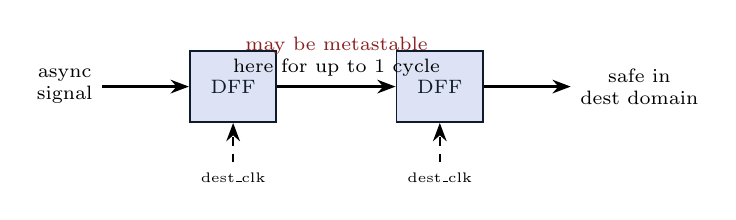
\begin{tikzpicture}[font=\scriptsize,
    ff/.style={draw=Navy,fill=BlueF,minimum height=0.9cm,minimum width=1.1cm,
      text=Navy,line width=0.7pt},
    >=Stealth]
  \node[ff] (F1) {DFF};
  \node[ff, right=1.5cm of F1] (F2) {DFF};
  \node[align=center, left=1.1cm of F1] (in) {async\\signal};
  \node[align=center, right=1.1cm of F2] (out) {safe in\\dest domain};
  \draw[->,thick] (in) -- (F1);
  \draw[->,thick] (F1) -- node[above,align=center]{\color{Red}may be metastable\\here for up to 1 cycle}(F2);
  \draw[->,thick] (F2) -- (out);
  \draw[->,thick,dashed] ($(F1.south)+(0,-0.5)$) node[below,font=\tiny]{dest\_clk} -- (F1.south);
  \draw[->,thick,dashed] ($(F2.south)+(0,-0.5)$) node[below,font=\tiny]{dest\_clk} -- (F2.south);
\end{tikzpicture}
\end{center}
\begin{center}
\parbox{0.85\linewidth}{\footnotesize\color{MGray}
Both flops are clocked by the \emph{destination} domain's clock. The first
flop is the one allowed to go metastable (its input crossed domains with no
timing relationship to \texttt{dest\_clk}); the second flop samples the
first flop's output one full \texttt{dest\_clk} period later, by which time
the exponential settling of Figure~1 has, overwhelmingly, already resolved
it to a valid rail.}
\end{center}

\begin{keybox}
Noise (thermal, supply, coupling) is exactly what nudges a flip-flop that
landed \emph{exactly} on the metastable balance point to one side or the
other — that's why the failure mode is sometimes phrased as "noise can
flip the bit": it's not corrupting a settled value, it's tipping an
\emph{unsettled} one, and which way it tips is genuinely unpredictable
from outside the device.
\end{keybox}

\subsection{Why a multi-bit bus needs Gray code, not just more sync flops}

Adding a second synchronizer flop fixes metastability \emph{per bit}. It
does \emph{not} fix a different, second problem that only shows up on
\textbf{multi-bit buses}: a plain binary counter can change \textbf{many
bits at once} on a single increment (e.g.\ \texttt{0111} $\to$
\texttt{1000} flips all 4 bits). Each of those bits is physically routed
on its own wire, with its own independent (if nominally identical) delay,
and is sampled by its own independent synchronizer flip-flop pair.

\begin{warnbox}
If the destination-domain clock edge lands \emph{during} that multi-bit
transition, different bits can be captured on different sides of their own
individual switching point — some already updated, some still showing the
old value. The captured word can then be \emph{any} combination of old and
new bits, including values the counter \textbf{never actually held}, e.g.\
sampling \texttt{0111}$\to$\texttt{1000} mid-flight could yield
\texttt{1111} or \texttt{0000} — a wildly wrong pointer value, not merely a
"stale by one" value.
\end{warnbox}

\textbf{Gray code} is the fix: it's a counting sequence in which
\textbf{exactly one bit changes between any two consecutive values}. With
only one bit ever in flight, the worst a torn sample can be is "the old
value" or "the new value" — \emph{never} anything else, because there is no
third combination available when only 1 bit differs. That's a 1-cycle
\emph{ambiguity} (which of the two adjacent, both-valid values did the
receiver see), not a \emph{corruption} (a value that was never real). The
FIFO's read and write pointers are therefore always converted to Gray code
\emph{before} crossing domains (and converted back after), specifically so
the multi-bit CDC only ever risks that benign 1-of-two ambiguity.

\begin{center}
\renewcommand{\arraystretch}{1.15}
\begin{tabular}{cccc}
\toprule
Decimal & Binary & Gray & Bits changed vs. previous \\
\midrule
0 & 000 & 000 & --  \\
1 & 001 & 001 & 1 \\
2 & 010 & 011 & 1 \\
3 & 011 & 010 & 1 \\
4 & 100 & 110 & 1 \\
5 & 101 & 111 & 1 \\
6 & 110 & 101 & 1 \\
7 & 111 & 100 & 1 \\
\bottomrule
\end{tabular}
\end{center}
Conversion is trivial and combinational: $\text{gray} = \text{bin} \oplus
(\text{bin} \gg 1)$, so it costs nothing beyond the synchronizer flops
already required.

\clearpage
% ============================================================
\section{Reader behavior: always-ready, sometimes-ready, never-ready}
\label{sec:readerbehavior}
% ============================================================

The credit scheme's job is to make all three of these safe and simple by
construction — the sender never special-cases any of them, it only ever
watches its own counter.

\begin{casebox}{Reader always ready (drains every cycle it can)}
\begin{center}
\begin{tikztimingtable}[timing/rowdist=2.6ex, timing/wscale=0.85]
  clk          & 8{C} \\
  push         & 8H \\
  pop          & 8H \\
  credit\_ret(+2) & 2L 6H \\
  credit\_cnt  & D{D}D{D-1}D{D-2}D{D-2}D{D-2}D{D-2}D{D-2}D{D-2} \\
\end{tikztimingtable}
\end{center}
Steady state: counter settles at $D - \text{RTT}$ and holds there,
sustaining full 1/cycle throughput indefinitely.
\end{casebox}

\begin{casebox}{Reader never ready (stalled, e.g.\ downstream backpressure)}
\begin{center}
\begin{tikztimingtable}[timing/rowdist=2.6ex, timing/wscale=0.85]
  clk          & 8{C} \\
  push         & 5H 3L \\
  pop          & 8L \\
  credit\_ret  & 8L \\
  credit\_cnt  & D{D}D{D-1}D{D-2}D{D-3}D{D-4}D{0}D{0}D{0} \\
\end{tikztimingtable}
\end{center}
Counter monotonically drains to 0 as the sender keeps pushing with no pops
occurring; once it hits 0, \texttt{push} correctly deasserts (sender
self-throttles). \textbf{This is correct, lossless backpressure} — data is
never dropped, the sender simply runs out of credit exactly when the
physical FIFO runs out of room, because $D$ was sized to make those two
events coincide.
\end{casebox}

\begin{casebox}{Reader sometimes ready (bursty consumption)}
\begin{center}
\begin{tikztimingtable}[timing/rowdist=2.6ex, timing/wscale=0.85]
  clk          & 10{C} \\
  push         & 10H \\
  pop          & 2H 3L 2H 3L \\
  credit\_ret(+2) & 4L 2H 3L 2H \\
  credit\_cnt  & D{4}D{3}D{2}D{1}D{2}D{2}D{2}D{1}D{2}D{2} \\
\end{tikztimingtable}
\end{center}
Counter free-runs between whatever bursts of pops/returns occur; as long as
it never needs to go below 0 (i.e.\ $D$ was sized for the worst-case burst
gap, not just the average rate), the sender never has to know or care that
the reader's cadence is irregular. \textbf{This is the real payoff of the
credit model}: the sender's logic is identical in all three of these
scenarios; only the counter's trajectory differs.
\end{casebox}

\subsection{This is not a niche technique}

Credit-based flow control under exactly this "sender counts, receiver
pulses" shape is the standard mechanism, not a one-off trick invented for
this FIFO:

\begin{itemize}[leftmargin=1.4em]
  \item \textbf{PCI Express} link-layer flow control works this way: each
  side advertises an initial credit allocation per traffic class at link
  init, the transmitter decrements local credit counters per TLP sent, and
  the receiver returns credit \emph{update} DLLPs as buffer space frees —
  structurally identical to Section~1's counter/pulse split, just at the
  packet-link layer instead of the RTL-clock layer.
  \item \textbf{Network-on-chip (NoC) routers} between IP blocks on the
  same die almost universally use per-virtual-channel credit counters
  precisely because the router-to-router hops are pipelined (multi-cycle),
  making plain valid/ready's round-trip-buffering cost (Case~6) prohibitive
  at every hop.
  \item \textbf{AXI} itself is valid/ready at the protocol boundary, but
  any AXI \emph{interconnect} with internal pipelining (which all
  non-trivial ones have) is typically implemented internally with
  credit-like skid/store-and-forward buffering precisely to present a
  compliant valid/ready face at the boundary while not paying Case~6's
  penalty internally — i.e.\ the credit discipline often lives just
  \emph{inside} the block, converted back to valid/ready only at the
  externally visible ports.
\end{itemize}

This is worth knowing mainly so the pattern is recognizable later: any time
"advertise capacity once, then count pulses" shows up, it's this same
tradeoff being made again.

\clearpage
% ============================================================
\section{Frequently confused points}
% ============================================================

A handful of questions that tend to come up once the mechanism above makes
sense on paper but before it's fully internalized.

\begin{description}[leftmargin=1.2em, style=nextline]
\item[\normalfont\bfseries "Isn't a credit pulse just a delayed \texttt{ready}?"]
No — the difference is not \emph{when} information arrives, it's \emph{what
the sender does while waiting for it}. A registered \texttt{ready} makes
the sender's \emph{next send decision} depend on a signal that is stale by
construction; the sender must either stall or risk Case~3/4's overrun. A
credit counter makes the sender's send decision depend only on \emph{its
own} state, which was correct at reset and is provably kept correct by the
invariant "counter $=$ physical free slots $-$ in-flight, unacknowledged
credit." The pulse's arrival \emph{updates} that local state; it is never
consulted live as a permission signal the way \texttt{ready} is.

\item[\normalfont\bfseries "Why not just make the skid buffer as deep as
needed at every stage, and keep valid/ready?"]
You could, and Case~6's formula tells you exactly how deep each one needs
to be. The credit/FIFO scheme isn't doing anything a correctly-sized
per-stage skid buffer chain couldn't do — it is simply
\emph{centralizing} that same storage into one place with one size
parameter, instead of re-deriving and re-verifying a skid depth at every
pipeline stage independently, and instead of paying for $N$ separate small
buffers when one buffer of the same total depth does the same job.

\item[\normalfont\bfseries "Does the credit scheme make the round-trip
latency disappear?"]
No. \textbf{Latency is physical and unavoidable} — Section~\ref{sec:trace}
still shows a full RTT of fill time before steady state, and the very
first word pushed still takes RTT cycles of wall-clock time before it's
possible for the receiver to signal anything about it back. What the
scheme eliminates is \emph{stalling due to not knowing the answer yet} —
sustained throughput, not first-word latency.

\item[\normalfont\bfseries "What if reset happens with credits already
in flight (a push sent, but its matching \texttt{credit\_ret} hasn't
arrived yet)?"]
This is exactly why both clock domains' resets, and the synchronizer
chains inside \texttt{pulse\_sync}, must be considered together
(Section~\ref{sec:verify}'s reset-skew checklist item). The safe pattern is: on any
reset of \emph{either} domain, reset the whole FIFO (\texttt{wptr},
\texttt{rptr}, and every synchronizer flop) back to empty in \emph{both}
domains via each domain's own reset, and re-initialize
\texttt{credit\_cnt} to $D$ only after both domains are confirmed out of
reset — never assume in-flight credits "settle out" on their own across
an asynchronous reset.

\item[\normalfont\bfseries "Can \texttt{credit\_cnt} ever legitimately
exceed $D$?"]
No, and if simulation ever shows it happening, that is a bug, not a corner
case: it means a \texttt{credit\_ret} pulse arrived that doesn't correspond
to a push that was ever actually granted (a spurious or duplicated pulse,
most likely a \texttt{pulse\_sync} edge-detection bug). This is exactly
the invariant the verification checklist's "credit accounting closure"
item (Section~\ref{sec:verify}) is designed to catch.
\end{description}

\clearpage
% ============================================================
\section{Summary cheat-sheet}
% ============================================================

\begin{center}
\renewcommand{\arraystretch}{1.3}
\begin{tabular}{@{}p{4.3cm}p{5.4cm}p{5.4cm}@{}}
\toprule
& \textbf{Valid/Ready} & \textbf{Valid/Credit} \\
\midrule
What crosses the round trip & live receiver state (or a stale registered
copy of it) & a single-bit "I freed a slot" pulse \\
What absorbs latency & nothing, by default -- must add matching skid
buffers at every registered stage & one counter, pre-loaded with the FIFO
depth at reset \\
Cost of extra pipeline stages & a new skid buffer decision at every stage,
every time & one number (depth) goes up, once \\
Under-sizing failure & throughput loss (safe, just slow) if conservative;
data overrun if not & data overrun (write pointer laps read pointer) --
must size correctly, no "safe-but-slow" fallback \\
Over-sizing cost & N/A (you'd just not add the stage) & silicon area only,
zero bandwidth cost \\
Scales to deep pipelines? & poorly -- distributed buffering decisions & yes
-- centralized, one depth parameter \\
\bottomrule
\end{tabular}
\end{center}

\begin{formulabox}
\textbf{Depth sizing, final form:}
\[
D_{\min} = \left\lceil \underbrace{2\cdot\tfrac{T_{rclk}}{T_{wclk}} + N_{read\_pipe}\cdot\tfrac{T_{rclk}}{T_{wclk}}}_{\text{read-domain latency, in wclk units}} + \underbrace{2 + N_{write\_pipe}}_{\text{write-domain latency}} \right\rceil + 1
\]
Round \emph{up} to the next power of 2 if the pointer/Gray-code scheme
requires it. Pointer width $= \lceil \log_2 D \rceil + 1$ bits (the extra
bit per Section~\ref{sec:pointer}).
\end{formulabox}

\clearpage
% ============================================================
\section{Reference SystemVerilog skeleton}
% ============================================================
Structure only -- for orienting yourself in an implementation, not a
tutorial on how to write SystemVerilog. Standard dual-pointer / Gray-code /
2-flop-synchronizer async FIFO core (per the reference article), with the
credit-counter and single-pulse credit-return layered on the write side.

\begin{lstlisting}[style=sv,caption={Async FIFO core: memory + Gray pointers + synchronizers}]
module async_fifo #(
  parameter DW = 32,
  parameter N  = 4              // depth = 2**N
)(
  input  logic            wclk, wrst_n,
  input  logic            wr_en,
  input  logic [DW-1:0]   wdata,
  output logic            full,

  input  logic            rclk, rrst_n,
  input  logic            rd_en,
  output logic [DW-1:0]   rdata,
  output logic            empty
);
  logic [N:0] wptr_bin, wptr_gray, wptr_gray_rsync1, wptr_gray_rsync2;
  logic [N:0] rptr_bin, rptr_gray, rptr_gray_wsync1, rptr_gray_wsync2;
  logic [DW-1:0] mem [0:(1<<N)-1];

  // -- write side --
  always_ff @(posedge wclk or negedge wrst_n)
    if (!wrst_n) wptr_bin <= '0;
    else if (wr_en && !full) begin
      mem[wptr_bin[N-1:0]] <= wdata;
      wptr_bin             <= wptr_bin + 1'b1;
    end
  assign wptr_gray = wptr_bin ^ (wptr_bin >> 1);   // bin->gray, combinational

  // 2-flop synchronizer, read ptr into write domain
  always_ff @(posedge wclk or negedge wrst_n)
    if (!wrst_n) {rptr_gray_wsync2, rptr_gray_wsync1} <= '0;
    else         {rptr_gray_wsync2, rptr_gray_wsync1}
                   <= {rptr_gray_wsync1, rptr_gray};

  assign full = (wptr_gray[N]   != rptr_gray_wsync2[N]) &&
                (wptr_gray[N-1] != rptr_gray_wsync2[N-1]) &&
                (wptr_gray[N-2:0] == rptr_gray_wsync2[N-2:0]);
  // (N:N-1 inverted-pair check is one common full-detect form for Gray
  //  pointers; equivalent to the wrap-bit compare shown in Sec. 4)

  // -- read side --
  always_ff @(posedge rclk or negedge rrst_n)
    if (!rrst_n) rptr_bin <= '0;
    else if (rd_en && !empty) rptr_bin <= rptr_bin + 1'b1;
  assign rptr_gray = rptr_bin ^ (rptr_bin >> 1);
  assign rdata      = mem[rptr_bin[N-1:0]];

  always_ff @(posedge rclk or negedge rrst_n)
    if (!rrst_n) {wptr_gray_rsync2, wptr_gray_rsync1} <= '0;
    else         {wptr_gray_rsync2, wptr_gray_rsync1}
                   <= {wptr_gray_rsync1, wptr_gray};

  assign empty = (rptr_gray == wptr_gray_rsync2);
endmodule
\end{lstlisting}

\begin{lstlisting}[style=sv,caption={Write-side credit counter + read-side credit-return pulse (layered on top of the core above)}]
module credit_push #(parameter D = 16)(
  input  logic wclk, wrst_n,
  input  logic push_req,        // sender wants to send
  output logic push_gnt,        // == wr_en into async_fifo
  input  logic credit_ret_pulse // synchronized, 1-cycle wide, from read side
);
  logic [$clog2(D):0] credit_cnt;   // note: extra bit, mirrors Sec. 4 logic
  assign push_gnt = push_req && (credit_cnt != '0);

  always_ff @(posedge wclk or negedge wrst_n)
    if (!wrst_n) credit_cnt <= D[$clog2(D):0];
    else begin
      unique case ({push_gnt, credit_ret_pulse})
        2'b10:   credit_cnt <= credit_cnt - 1'b1;
        2'b01:   credit_cnt <= credit_cnt + 1'b1;
        default: credit_cnt <= credit_cnt; // 00: no change, 11: net zero
      endcase
    end
endmodule

module credit_return (
  input  logic rclk, rrst_n,
  input  logic pop_event,          // 1 cycle, asserted when a pop retires
  output logic credit_ret_pulse_r  // still in rclk domain; sync into wclk
                                    // with a 2-flop pulse synchronizer
                                    // (toggle + edge-detect, or a small
                                    // async FIFO of its own) before use
                                    // above.
);
  assign credit_ret_pulse_r = pop_event;
endmodule
\end{lstlisting}

\noindent Note the \texttt{2'b11} case in \texttt{credit\_push}: a push and
a credit-return can legitimately land on the sender's clock in the same
cycle (the return pulse arrived from a pop that happened up to
$\text{RTT}$ cycles ago, unrelated to whatever the sender is doing right
now) — net effect on the counter is zero, which is exactly why
\emph{simultaneous} alloc+retire must never be treated as "no event," only
as "both events, which happen to cancel."

\subsection{Closing the gap: the pulse synchronizer}
\label{sec:pulsesync}

\texttt{credit\_return} above hands off a single-cycle \texttt{rclk} pulse;
it cannot be sent through a plain 2-flop synchronizer as-is, because a
1-cycle-wide pulse in a \emph{faster} \texttt{rclk} domain can fall entirely
inside one \texttt{wclk} period and be missed by a slower sampling clock
(the classic "pulse too narrow to be seen" CDC bug — unrelated to
metastability, and just as fatal). The standard fix is a
\textbf{toggle-and-resynchronize} pulse synchronizer: convert the pulse to
a level (toggle a flip-flop on every pop), synchronize that \emph{level}
with an ordinary 2-flop synchronizer (levels, unlike pulses, cannot be
"missed" — whatever value it's at, it stays there until the next toggle),
then edge-detect the synchronized level back into a clean 1-cycle pulse in
the destination domain.

\begin{lstlisting}[style=sv,caption={Toggle-based pulse synchronizer: rclk pulse -> wclk pulse}]
module pulse_sync (
  input  logic src_clk, src_rst_n,
  input  logic pulse_in,        // 1-cycle wide, src_clk domain
  input  logic dst_clk, dst_rst_n,
  output logic pulse_out        // 1-cycle wide, dst_clk domain
);
  logic toggle_src;
  logic toggle_dst_s1, toggle_dst_s2, toggle_dst_s3;

  // source domain: pulse -> toggle (a level, safe to synchronize)
  always_ff @(posedge src_clk or negedge src_rst_n)
    if (!src_rst_n) toggle_src <= 1'b0;
    else if (pulse_in) toggle_src <= ~toggle_src;

  // destination domain: 2-flop sync + 1 extra flop for edge detect
  always_ff @(posedge dst_clk or negedge dst_rst_n)
    if (!dst_rst_n) {toggle_dst_s3, toggle_dst_s2, toggle_dst_s1} <= '0;
    else {toggle_dst_s3, toggle_dst_s2, toggle_dst_s1}
           <= {toggle_dst_s2, toggle_dst_s1, toggle_src};

  assign pulse_out = toggle_dst_s2 ^ toggle_dst_s3;  // edge = level changed
endmodule
\end{lstlisting}

This is the piece that actually sits in the "S--S" boxes of the system
block diagram in Section~1.1, and it is also the standard building block
for crossing the Gray-coded pointers themselves in Section~\ref{sec:pointer}
when the design instead chooses to compare pointers directly rather than
count discrete credits — the two schemes (direct pointer compare vs.\
credit count) are two ways of asking the same underlying question
("how much room is left"), and both bottom out in exactly this
toggle-synchronize-edge-detect primitive, or the level-based 2-flop
synchronizer of Section~\ref{sec:cdc} when what's crossing is already a
level (like a Gray pointer bit) rather than a pulse.

\subsection{Top-level: wiring the pieces together}

The four pieces above (\texttt{async\_fifo}, \texttt{credit\_push},
\texttt{credit\_return}, \texttt{pulse\_sync}) are never useful in
isolation — this is how they compose into the single block from the
system diagram in Section~1.1.

\begin{lstlisting}[style=sv,caption={Top-level: async FIFO + credit-based push/pop, both domains}]
module credit_fifo_top #(
  parameter DW = 32,
  parameter N  = 3            // depth D = 2**N = 8
)(
  input  logic            wclk, wrst_n,
  input  logic            push_req,
  output logic            push_gnt,
  input  logic [DW-1:0]   wdata,

  input  logic            rclk, rrst_n,
  input  logic            rd_en,
  output logic [DW-1:0]   rdata,
  output logic            rvalid        // == !empty, exposed for convenience
);
  localparam int D = (1 << N);

  logic wr_en, full, empty, pop_event, credit_ret_w;

  assign wr_en     = push_gnt;                 // push_gnt already checked credit
  assign pop_event = rd_en && !empty;
  assign rvalid    = !empty;

  async_fifo #(.DW(DW), .N(N)) u_fifo (
    .wclk(wclk), .wrst_n(wrst_n), .wr_en(wr_en), .wdata(wdata), .full(full),
    .rclk(rclk), .rrst_n(rrst_n), .rd_en(rd_en), .rdata(rdata), .empty(empty)
  );

  credit_push #(.D(D)) u_credit_push (
    .wclk(wclk), .wrst_n(wrst_n),
    .push_req(push_req), .push_gnt(push_gnt),
    .credit_ret_pulse(credit_ret_w)
  );

  pulse_sync u_credit_sync (
    .src_clk(rclk), .src_rst_n(rrst_n), .pulse_in(pop_event),
    .dst_clk(wclk), .dst_rst_n(wrst_n), .pulse_out(credit_ret_w)
  );
endmodule
\end{lstlisting}

Two details worth flagging explicitly, since they are the kind of thing
that's obvious once pointed out and easy to miss otherwise:

\begin{itemize}[leftmargin=1.4em]
  \item \texttt{full} (from \texttt{async\_fifo}) is deliberately
  \textbf{unused} by \texttt{wr\_en} here — the credit counter is the sole
  authority on whether a push is allowed, by design (Section~1). If
  \texttt{full} and \texttt{credit\_cnt} ever disagree in simulation, that
  disagreement — not a wire you'd reach for to "fix" the symptom — is the
  bug to chase (this is exactly the invariant the verification checklist's
  "credit accounting closure" item polices).
  \item \texttt{credit\_ret\_w} both feeds \texttt{credit\_push} as an
  input and is driven as \texttt{pulse\_sync}'s output — a normal
  same-cycle net, not a combinational loop, because it crosses from
  \texttt{rclk} to \texttt{wclk} through registered synchronizer stages;
  there is no path from \texttt{credit\_push}'s output back into
  \texttt{pulse\_sync}'s input.
\end{itemize}

\clearpage
% ============================================================
\section{Verification checklist}
\label{sec:verify}
% ============================================================

Practical checklist for a testbench exercising this design — each item
targets one failure mode analyzed above, not generic FIFO sanity.

\begin{enumerate}[leftmargin=1.4em]
  \item \textbf{Max-rate sweep across clock ratios.} Run back-to-back
  pushes at \texttt{credit\_cnt}$>0$ for every ratio in the sizing sweep
  table (Section~\ref{sec:sizing}), including non-integer ratios — confirm
  \texttt{full} is never asserted incorrectly and no data is dropped.
  \item \textbf{$D_{\min}-1$ regression.} Deliberately build the design one
  entry shallower than the sizing formula recommends and confirm the
  testbench \emph{catches} the Case~10 overrun (a scoreboard mismatch or an
  assertion on write-while-full) — if under-sizing doesn't fail visibly in
  simulation, the checker itself is the bug.
  \item \textbf{Pulse-width-1 guarantee.} Assert, on both sides of every
  \texttt{pulse\_sync} instance, that \texttt{pulse\_in}/\texttt{pulse\_out}
  are never asserted for more than 1 destination-clock cycle, and that
  back-to-back toggles (two pops on adjacent source cycles) are not merged
  into one destination pulse or dropped.
  \item \textbf{Reset behavior.} Assert both \texttt{wrst\_n} and
  \texttt{rrst\_n} independently and skewed in time (real designs don't
  reset both domains synchronously); confirm pointers, \texttt{credit\_cnt},
  and both synchronizer chains all return to a consistent empty state with
  no spurious \texttt{credit\_ret} pulses generated by the toggle flops
  glitching through reset.
  \item \textbf{Simultaneous full+empty edge.} Drive push and pop on the
  exact same cycle when the FIFO has exactly 1 entry — confirm neither
  \texttt{full} nor \texttt{empty} glitches, and the Gray-pointer
  full/empty compare (Section~\ref{sec:pointer}) resolves correctly on both
  domains' next sample.
  \item \textbf{Gray-code wraparound.} Force the pointers through several
  full wraps (push/pop counts $\gg 2^{N}$) and confirm the wrap-bit compare
  keeps distinguishing full from empty correctly lap after lap — this is
  the one most likely to silently regress if someone "simplifies" the
  pointer width back to \texttt{[N-1:0]}.
  \item \textbf{Credit accounting closure.} Over a long random run, assert
  $\text{pushes} - \text{pops} = D - \text{credit\_cnt}$ at every cycle (in
  the write domain) — any divergence means a credit event was double-
  counted or dropped, independent of whether data corruption is visible
  yet.
  \item \textbf{All three reader profiles.} Replay the always-ready,
  never-ready, and bursty-sometimes-ready scenarios from
  Section~\ref{sec:readerbehavior} back to back in one run (not three
  separate tests) to catch state left over from one profile corrupting
  the next.
\end{enumerate}

\clearpage
% ============================================================
\section*{Glossary}
\addcontentsline{toc}{section}{Glossary}
% ============================================================

\begin{description}[leftmargin=3.2cm, style=nextline]
\item[valid] Sender-asserted signal: "the data on this bus is real, right
  now."
\item[ready] Receiver-asserted signal: "I can accept a transfer, right
  now." A transfer occurs exactly when both are 1 on the same clock edge.
\item[credit] A token representing one free slot of storage somewhere
  downstream; the sender is authorized to send exactly as many outstanding
  items as it holds credits for.
\item[credit return / credit\_ret] The single-cycle pulse the receiver
  sends upstream each time it frees one slot (typically: each pop).
\item[skid buffer] A small amount of extra storage added at a pipeline
  stage specifically to hold data that was already committed to move
  before the stage learned the downstream side wasn't ready.
\item[round-trip time (RTT)] The number of cycles between a sender's
  action and the earliest cycle that action's consequence could possibly
  be reflected back to the sender.
\item[CDC] Clock domain crossing: any signal path between two flip-flops
  clocked by clocks with no fixed phase relationship.
\item[metastability] A flip-flop's internal storage node settling near an
  indeterminate voltage instead of resolving cleanly to a valid logic
  level within one clock period, because its setup/hold window was
  violated.
\item[MTBF] Mean time between (synchronizer) failures — the expected time
  before a metastable event fails to resolve within the allotted
  settling time and propagates a bad value.
\item[2-flop synchronizer] Two flip-flops in series, both clocked by the
  destination domain, used to give a crossing signal one full clock
  period of settling time before it's used.
\item[Gray code] A binary encoding in which consecutive values differ in
  exactly one bit, used for any multi-bit counter/pointer that must cross
  a clock domain.
\item[wrap bit] The extra, $(N{+}1)^{\text{th}}$, bit carried by FIFO
  read/write pointers (beyond the $N$ bits needed to index the memory)
  that disambiguates "just wrapped around" from "never wrapped," and
  therefore full from empty.
\item[full / empty] FIFO status flags: \texttt{empty} when the (synced)
  write pointer equals the read pointer including the wrap bit;
  \texttt{full} when the bottom $N$ bits match but the wrap bits differ.
\end{description}

\end{document}
